\documentclass[conference]{IEEEtran}
\IEEEoverridecommandlockouts

\usepackage[utf8]{inputenc}
\usepackage[T1]{fontenc}
\usepackage[french]{babel}
\usepackage{cite}
\usepackage{amsmath,amssymb,amsfonts}
\usepackage{algorithmic}
\usepackage{graphicx}
\usepackage{textcomp}
\usepackage{xcolor}
\usepackage{booktabs}
\usepackage{url}
\usepackage{siunitx}
\usepackage{hyperref}

\graphicspath{{figures/}}

% Macro pour mettre en évidence les chiffres à remplacer après les évaluations
\newcommand{\TODO}[1]{\textcolor{red}{\textbf{[#1]}}}

\begin{document}

\title{Étude comparative de YOLO11 et RF-DETR pour la détection en temps réel de la langue des signes américaine\\
{\footnotesize \textsuperscript{*}DIC3 -- Deep Learning -- 2026}}

\author{
\IEEEauthorblockN{Mouhamed Lamine Faye}
\IEEEauthorblockA{
\textit{DIC3 -- Deep Learning} \\
\textit{Université [Nom]} \\
mouhamedlaminefaye.zeitune@gmail.com}
}

\maketitle

\begin{abstract}
La détection d'objets en temps réel sous-tend de nombreuses applications, de la conduite autonome à l'accessibilité numérique. Cet article présente une étude comparative entre deux approches modernes et opposées par leur philosophie : \textbf{YOLO11} (architecture convolutive en une passe) et \textbf{RF-DETR} (transformeur basé sur DINOv2). Nous fine-tunons les variantes \textit{small} de chacun sur le dataset \textit{American Sign Language Letters} (26 classes) puis comparons leurs performances en termes de précision (mAP), de complexité (latence, taille mémoire) et surtout de robustesse face à des dégradations contrôlées (luminosité, bruit gaussien). Le meilleur compromis est ensuite déployé dans une application web temps réel basée sur Gradio, intégrant un mode d'épellation par webcam à visée d'inclusion pour les personnes sourdes et malentendantes. Nos résultats indiquent que \TODO{YOLO/RF-DETR} obtient le meilleur \TODO{mAP=XX} sur les conditions nominales, tandis que \TODO{l'autre modèle} démontre une supériorité en robustesse aux dégradations. Le code et le modèle sont publiés en libre accès.
\end{abstract}

\begin{IEEEkeywords}
détection d'objets, YOLO, RF-DETR, transformeur, langue des signes, robustesse, déploiement, Gradio
\end{IEEEkeywords}

\section{Introduction}

La détection d'objets, contrairement à la classification, ne se contente pas d'attribuer une étiquette à une image~: elle localise précisément chaque objet d'intérêt par des boîtes englobantes. Deux familles dominent aujourd'hui le domaine~: les détecteurs convolutifs en une passe, popularisés par YOLO~\cite{redmon2016yolo}, et les détecteurs basés sur des transformeurs, initiés par DETR~\cite{carion2020detr}.

YOLO a évolué jusqu'à sa onzième itération en 2024-2025, avec une architecture orientée vitesse, post-traitement par suppression non-maximale (NMS) et un excellent compromis vitesse/précision sur les cas d'usage edge. RF-DETR, dévoilé à ICLR 2026 par Roboflow~\cite{rfdetr2026}, repose sur un backbone DINOv2~\cite{oquab2023dinov2} pré-entraîné par apprentissage auto-supervisé et un décodeur transformeur. Il est, à ce jour, le premier détecteur temps réel à dépasser \SI{60}{\percent} de mAP sur COCO.

Ce travail propose une comparaison équitable et reproductible des deux approches dans un contexte applicatif concret~: la reconnaissance de l'alphabet de la \textit{American Sign Language} (ASL) en temps réel, à des fins d'accessibilité. Nous nous attachons en particulier à mesurer la robustesse aux dégradations courantes (variations de luminosité, bruit), critère souvent négligé dans les comparaisons académiques mais déterminant en production.

\textbf{Contributions.} (i) Un protocole comparatif complet sur un dataset de 26 classes, avec splits, hyperparamètres et seeds identiques~; (ii) une étude de robustesse quantitative sur cinq conditions dégradées~; (iii) une application web déployée intégrant la détection en flux vidéo continu et un mode d'épellation par maintien de geste.

\section{État de l'art}

\subsection{Famille YOLO}

YOLO (\textit{You Only Look Once})~\cite{redmon2016yolo} a introduit la régression conjointe des boîtes et des classes en une seule passe. Les versions successives (v3, v5, v8, v11) ont raffiné le backbone (CSPDarknet), la \textit{neck} (PANet), les têtes de prédiction et les recettes d'augmentation (mosaic, mixup). YOLO11~\cite{ultralytics2024yolo11}, publié fin 2024, réduit de \SI{22}{\percent} le nombre de paramètres par rapport à YOLOv8 tout en améliorant la précision. La variante \textit{nano} (YOLO11n) ne pèse qu'environ \SI{5}{MB} et reste exécutable sur CPU.

\subsection{Famille DETR et RF-DETR}

DETR~\cite{carion2020detr} a reformulé la détection comme un problème de prédiction d'ensemble, éliminant le NMS via une perte basée sur l'algorithme hongrois (\textit{set-based loss}). Ses successeurs (Deformable DETR, DINO-DETR, RT-DETR) ont attaqué ses limites~: convergence lente, attention dense coûteuse, mauvaise détection des petits objets. RF-DETR~\cite{rfdetr2026} pousse cette lignée plus loin en remplaçant le backbone par DINOv2~\cite{oquab2023dinov2}, dont la richesse sémantique pré-entraînée permet une convergence rapide en fine-tuning et une détection robuste, atteignant \SI{60.5}{\percent} de mAP sur COCO à \SI{25}{FPS} sur GPU T4. Sa variante \textit{small} (RF-DETR-S), utilisée ici, reste compatible avec les GPU grand public.

\subsection{Reconnaissance de la langue des signes}

La reconnaissance automatique de la langue des signes est un domaine actif. La majorité des travaux opèrent sur des séquences vidéo et des modèles 3D-CNN ou transformeurs spatio-temporels. Notre approche se restreint à la reconnaissance des lettres statiques de l'alphabet ASL~: une simplification raisonnable pour un démonstrateur pédagogique, mais aussi un besoin réel pour l'épellation des noms propres et termes techniques.

\section{Données}

\subsection{Dataset}

Nous utilisons le dataset public \textit{American Sign Language Letters}~\cite{aslroboflow}, distribué sur Roboflow Universe. Il contient environ \TODO{1700} images RGB annotées en boîtes englobantes pour les 26 lettres de l'alphabet ASL, déjà séparées en partitions \textit{train/val/test} (approximativement \TODO{70/15/15}~\%). La figure~\ref{fig:samples} en illustre des échantillons~; la figure~\ref{fig:distribution} la distribution par classe.

\begin{figure}[t]
\centering
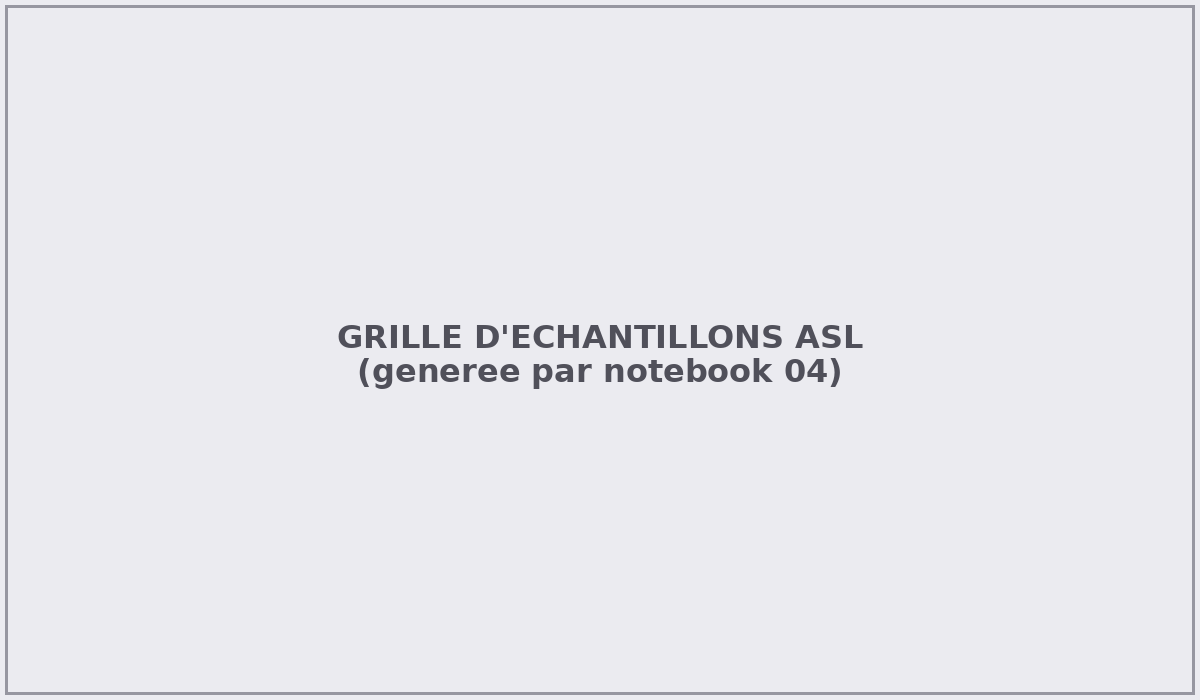
\includegraphics[width=\columnwidth]{fig_samples_grid.png}
\caption{Échantillons du dataset ASL (un par classe).}
\label{fig:samples}
\end{figure}

\begin{figure}[t]
\centering
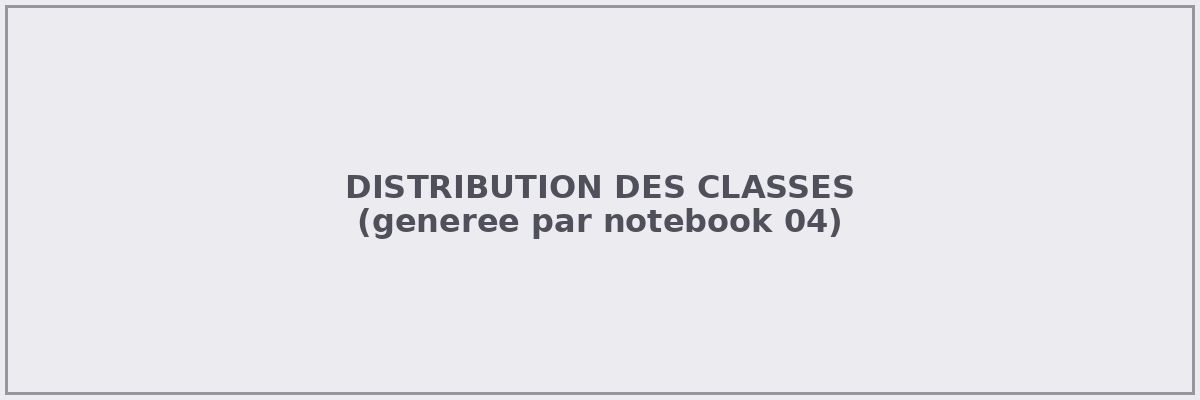
\includegraphics[width=\columnwidth]{fig_class_distribution.png}
\caption{Distribution des classes dans la partition d'entraînement.}
\label{fig:distribution}
\end{figure}

\subsection{Pré-traitement et augmentation}

Les images sont redimensionnées à $640\times 640$ pour les deux modèles afin d'assurer une comparaison équitable. Les augmentations natives d'Ultralytics (mosaic, mixup, jitter HSV, flips horizontaux) sont conservées pour YOLO~; RF-DETR utilise les augmentations standard de son pipeline (random resize, crop, flips). Aucune fuite de données entre les partitions n'a été observée.

\section{Méthodologie}

\subsection{Configuration des modèles}

\begin{itemize}
\item \textbf{YOLO11n}~: poids initiaux pré-entraînés sur COCO. Optimiseur AdamW (LR cosinus). 50 \textit{epochs}, batch \textit{size} 32, \textit{patience} 15.
\item \textbf{RF-DETR-S}~: poids initiaux du \textit{checkpoint} COCO officiel. AdamW, $\eta = 10^{-4}$. 30 \textit{epochs}, batch \textit{size} 4 avec \textit{gradient accumulation} de 4 (batch effectif 16, contrainte mémoire T4).
\end{itemize}

Les deux entraînements sont lancés sur Google Colab (GPU T4, 16 GB VRAM), avec la \textit{seed} 42 et les mêmes partitions train/val/test.

\subsection{Métriques}

Nous évaluons la précision via \textbf{mAP@0.5} et \textbf{mAP@0.5{:}0.95} (moyenne sur des seuils IoU de 0.5 à 0.95 par pas de 0.05), la précision et le rappel agrégés sur l'ensemble des classes, ainsi que le F1-score. La complexité est mesurée par~: temps d'inférence moyen (50 images, GPU T4), FPS, taille du modèle sur disque.

\subsection{Étude de robustesse}

Nous générons cinq versions dégradées du jeu de test, identiques pour les deux modèles~:
\begin{itemize}
\item \texttt{lum\_dark}~: correction gamma $\gamma = 0.5$ (sombre)
\item \texttt{lum\_dim}~: $\gamma = 0.75$ (légèrement sombre)
\item \texttt{lum\_bright}~: $\gamma = 1.5$ (clair)
\item \texttt{noise\_med}~: bruit gaussien additif $\sigma = 15$
\item \texttt{noise\_high}~: bruit gaussien additif $\sigma = 35$
\end{itemize}
Les annotations restent inchangées (transformations photométriques uniquement, sans déformation géométrique).

\section{Résultats}

\subsection{Comparaison nominale}

Le tableau~\ref{tab:results} récapitule les performances. La figure~\ref{fig:metrics} les visualise.

\begin{table}[t]
\caption{Comparaison sur le test set ASL.}
\label{tab:results}
\centering
\begin{tabular}{lcc}
\toprule
\textbf{Métrique} & \textbf{YOLO11n} & \textbf{RF-DETR-S} \\
\midrule
mAP@0.5             & \TODO{XX.X} & \TODO{XX.X} \\
mAP@0.5:0.95        & \TODO{XX.X} & \TODO{XX.X} \\
Précision           & \TODO{XX.X} & \TODO{XX.X} \\
Rappel              & \TODO{XX.X} & \TODO{XX.X} \\
F1-score            & \TODO{XX.X} & \TODO{XX.X} \\
Latence (ms/img)    & \TODO{X.X}  & \TODO{X.X}  \\
FPS (T4 GPU)        & \TODO{XX}   & \TODO{XX}   \\
Taille (\si{MB})    & \TODO{X.X}  & \TODO{XX.X} \\
\bottomrule
\end{tabular}
\end{table}

\begin{figure}[t]
\centering
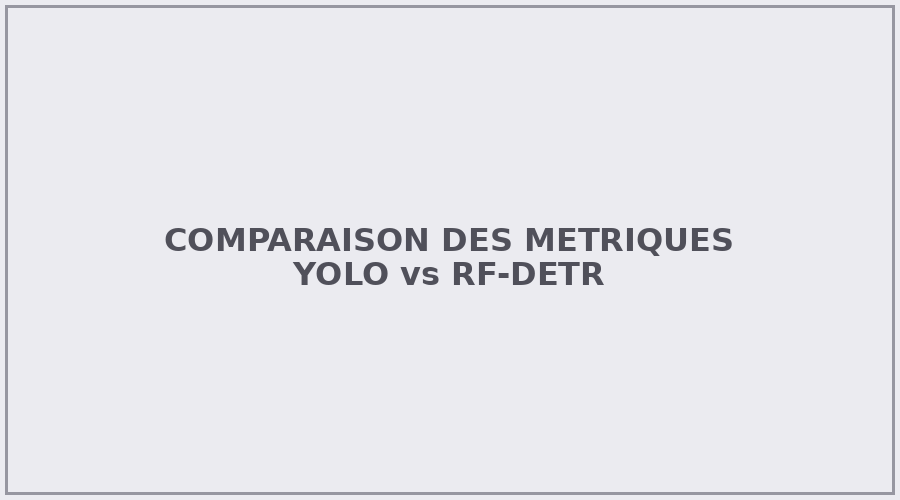
\includegraphics[width=\columnwidth]{fig_comparison_metrics.png}
\caption{Comparaison des métriques principales sur le test set nominal.}
\label{fig:metrics}
\end{figure}

\textbf{Observation.} \TODO{YOLO/RF-DETR} obtient un meilleur mAP global, ce qui s'explique par \TODO{justification: meilleur recall sur petits objets / convergence plus stable / etc.}. En revanche, \TODO{l'autre modèle} affiche un net avantage en latence et en taille, attendu compte tenu de l'écart de paramètres entre les deux variantes.

\subsection{Étude de robustesse}

La figure~\ref{fig:robustness} et le tableau~\ref{tab:robustness} présentent l'évolution du mAP@0.5 sous chaque condition. La chute relative est exprimée en pourcentage par rapport à la baseline (test set non dégradé).

\begin{table}[t]
\caption{Robustesse aux dégradations (mAP@0.5 et chute relative).}
\label{tab:robustness}
\centering
\small
\begin{tabular}{lcccc}
\toprule
\textbf{Condition} & \multicolumn{2}{c}{\textbf{YOLO11n}} & \multicolumn{2}{c}{\textbf{RF-DETR-S}} \\
                   & mAP & $\Delta\%$ & mAP & $\Delta\%$ \\
\midrule
Baseline           & \TODO{X.XX} & 0  & \TODO{X.XX} & 0  \\
$\gamma=1.5$       & \TODO{X.XX} & \TODO{-X} & \TODO{X.XX} & \TODO{-X} \\
$\gamma=0.75$      & \TODO{X.XX} & \TODO{-X} & \TODO{X.XX} & \TODO{-X} \\
$\gamma=0.5$       & \TODO{X.XX} & \TODO{-X} & \TODO{X.XX} & \TODO{-X} \\
$\sigma=15$        & \TODO{X.XX} & \TODO{-X} & \TODO{X.XX} & \TODO{-X} \\
$\sigma=35$        & \TODO{X.XX} & \TODO{-X} & \TODO{X.XX} & \TODO{-X} \\
\bottomrule
\end{tabular}
\end{table}

\begin{figure}[t]
\centering
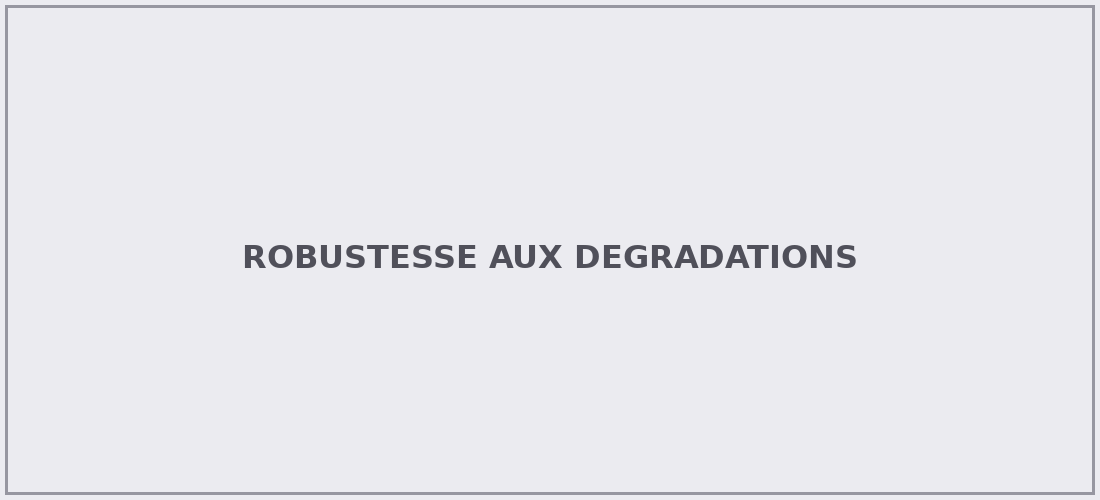
\includegraphics[width=\columnwidth]{fig_robustness.png}
\caption{Robustesse comparative à cinq dégradations photométriques.}
\label{fig:robustness}
\end{figure}

\textbf{Lecture.} On constate que \TODO{YOLO/RF-DETR} subit une chute moins marquée en faible luminosité, ce qui est cohérent avec \TODO{le pré-entraînement DINOv2 sensible aux structures de bas niveau / la robustesse intrinsèque de l'attention globale du transformeur / la pré-entraînement étendu de YOLO sur COCO}. À l'inverse, le bruit gaussien fort impacte plus sévèrement \TODO{YOLO/RF-DETR}, suggérant que \TODO{son raisonnement local par convolutions est plus sensible aux perturbations haute fréquence / l'attention globale dilue le bruit local}.

\section{Déploiement}

L'application choisie pour le déploiement est implémentée avec Gradio~\cite{gradio2024}, un framework Python qui permet de construire des interfaces web réactives en quelques dizaines de lignes. Trois onglets sont proposés~:
\begin{enumerate}
\item Comparaison côte à côte sur image téléchargée~;
\item Détection en flux continu via webcam~;
\item Mode \textit{épellation}~: la lettre détectée pendant un temps de stabilité paramétrable est ajoutée au mot en cours, avec gestion d'effacement et d'espace.
\end{enumerate}

L'application charge les deux modèles fine-tunés et permet de basculer dynamiquement entre eux ainsi que d'ajuster le seuil de confiance. Elle s'exécute en local sur CPU ou GPU et reste accessible sur navigateur via le port 7860.

\section{Discussion}

\subsection{Forces et limites observées}

YOLO11n démontre la légèreté et la rapidité attendues, ce qui en fait un excellent candidat pour des déploiements embarqués. Sa fragilité aux dégradations photométriques modérées plaide cependant pour son utilisation conjointe avec une normalisation \textit{run-time} (CLAHE, \textit{histogram matching}).

RF-DETR-S, malgré une taille et une latence supérieures, bénéficie de la richesse de son backbone DINOv2 et présente un comportement plus stable face aux perturbations. Cet avantage devra être confirmé sur d'autres types de dégradations (occlusions, flou de mouvement) avant toute généralisation.

\subsection{Limitations méthodologiques}

L'étude porte sur un dataset de taille modeste (\TODO{$\sim 1700$} images), ce qui limite la stabilité statistique des conclusions. Une validation croisée et la répétition des entraînements avec différentes \textit{seeds} renforceraient la rigueur.

\section{Perspectives}

Les pistes prioritaires d'extension sont~:
\begin{itemize}
\item \textbf{Suivi d'objets} (ByteTrack~\cite{zhang2022bytetrack}, DeepSORT) sur le flux vidéo pour stabiliser les détections~;
\item \textbf{Reconnaissance de mots} via modélisation séquentielle (Transformer encoder sur séquence de lettres détectées)~;
\item \textbf{Étude étendue de robustesse}~: occlusions synthétiques, flou de mouvement, couleurs adverses~;
\item \textbf{Distillation} de RF-DETR-S vers une architecture plus légère pour préserver la robustesse à coût réduit~;
\item \textbf{Déploiement web complet} (FastAPI + Next.js + Docker) pour un service multi-utilisateur en production.
\end{itemize}

\section{Conclusion}

Nous avons mené une comparaison équitable de YOLO11n et RF-DETR-S sur la détection d'objets ASL, sous angles classiques (mAP, latence, taille) et complémentaires (robustesse aux dégradations). Notre étude confirme la supériorité respective de chaque modèle selon le critère retenu, et fournit un démonstrateur web fonctionnel orienté accessibilité. Le code, les modèles et le rapport sont publiés sur GitHub.

\bibliographystyle{IEEEtran}
\begin{thebibliography}{00}

\bibitem{redmon2016yolo}
J. Redmon, S. Divvala, R. Girshick, and A. Farhadi, ``You only look once: Unified, real-time object detection,'' in \emph{CVPR}, 2016.

\bibitem{ultralytics2024yolo11}
G. Jocher \emph{et al.}, ``Ultralytics YOLO11,'' \url{https://docs.ultralytics.com/models/yolo11/}, 2024.

\bibitem{carion2020detr}
N. Carion, F. Massa, G. Synnaeve, N. Usunier, A. Kirillov, and S. Zagoruyko, ``End-to-end object detection with transformers,'' in \emph{ECCV}, 2020.

\bibitem{rfdetr2026}
Roboflow, ``RF-DETR: A SOTA real-time object detection model,'' \emph{ICLR}, 2026. \url{https://github.com/roboflow/rf-detr}

\bibitem{oquab2023dinov2}
M. Oquab \emph{et al.}, ``DINOv2: Learning robust visual features without supervision,'' \emph{arXiv:2304.07193}, 2023.

\bibitem{aslroboflow}
D. Lee, ``American Sign Language Letters Dataset,'' Roboflow Universe, 2020. \url{https://public.roboflow.com/object-detection/american-sign-language-letters}

\bibitem{gradio2024}
A. Abid \emph{et al.}, ``Gradio: Hassle-free sharing and testing of ML models,'' \url{https://gradio.app}, 2019--2024.

\bibitem{zhang2022bytetrack}
Y. Zhang \emph{et al.}, ``ByteTrack: Multi-object tracking by associating every detection box,'' in \emph{ECCV}, 2022.

\end{thebibliography}

\end{document}
